\documentclass[10pt]{•}\documentclass{report}
\usepackage[T1]{fontenc}
\usepackage{parskip}
\usepackage{graphicx}
\usepackage{fancyvrb}
\usepackage{hyperref}

\graphicspath{{./images/}}
\begin{document}
	\chapter{Introduction}
	\section{Just what is Angular?}
Angular is a framework for programming the web using components. The web componentization movement started a little while ago. Now, there are many serious players in this field, e.g., Angular, React, Svelte, Vue, just to name a few. The native web technologies (HTML, CSS, and JavaScript) have also started out in this direction by introducing the Web Components \href{https://www.webcomponents.org/specs}{specification}.

All these different libraries and frameworks have about the same concept of what constitutes a component. For example, an Angular component has all the necessary ingredients to make a chunk of HTML look and behave in a specific way wherever it's used. That's right! An Angular component can be tucked anywhere in a web page and still afford to look and behave consistently. That's pure reusability for you! How does it achieve that? An Angular component has all the required HTML, CSS, and JavaScript tightly encapsulated and is thus able to bring reusability to the table. Before diving into the details, let's get to see an Angular component in action!

Let's start by installing Node.js and the required NPM packages. I suggest using a node version manager like \href{https://github.com/jasongin/nvs}{NVS} to manage installations of different Node versions on your machine.

Install Node.js version 16.17+. Ensure that the version of NPM is 8.19+ and the browser is Chrome, version 100+.

When learning and working with Angular, \textsl{Angular CLI} is our best friend. \textsl{CLI} stands for \textsl{Command Line Interpreter}. We need to type in various commands on the command line to use the features of CLI, like e.g., creating a new Angular project, adding components to an existing one, etc. Each of these tasks involve writing some boiler-plate code which the CLI takes care. The CLI, thus makes it easy to work with Angular projects.

First, let's start by installing CLI using the command line\footnote{The version being installed here is 16.1.0. However, this command should also upgrade an older version of CLI if one's installed.}:

\texttt{npm install -g @angular/cli@16.1.0}

Next, let's create an Angular project using the newly installed CLI. The name of the project is \textsl{booklibrary}. Ensure there's no folder by that name and in the command line enter: 

\texttt{ng new booklibrary --prefix bk --defaults --standalone}

We have invoked the \verb|new| command of the CLI that takes care of creating an Angular project! After a few moments of entering those seemingly magic incantations, if everything goes well, we should be greeted by the message: 'Successfully initialized git.' and should see a new folder with the name \textsl{booklibrary} created. We are good to go! \verb|cd| into the folder and enter:

\texttt{ng serve}

After a few moments, We should see the message: \textbf{\texttt{Angular Live Development Server is listening on localhost:4200}}. Open \url{http://localhost:4200} in a browser and, lo! we should see our very first web app up and running!

What magic did the CLI perform to bring up the web app? Let's investigate starting from the \textsl{booklibrary} folder that was created by the \verb|ng new| command! There should be files in that folder as shown in the figure below:

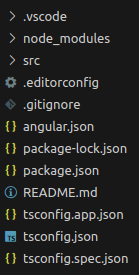
\includegraphics[scale=0.5]{project-structure}

These files were created by the \verb|ng new| command and constitute the Angular project. Among the files there's a \textsl{package.json} file that defines the \textsl{npm packages} that the project depends on. The important dependencies are:

\begin{itemize}
	\item @angular packages, the main libraries that constitute the Angular framework.
	\item rxjs - a library that makes it convenient to work with Observables.
	\item zone.js - a library for change detection; a core function required by Angular framework.
	\item dependencies for developing the application like Angular CLI, Typescript compiler, Jasmine unit testing tool, etc.
\end{itemize}

Other files of interest in the project are
\begin{itemize}
	\item \textsl{angular.json}. Angular specific project settings are stored here.
	\item The Typescript compiler has its own configuration files in the project folder named \textsl{tsconfig.json} and \textsl{tsconfig.app.json}. They store options required by the Typescript compiler, like e.g., an option for generating source maps\footnote{Source maps allow us to debug our app in the browser's dev console with the original Typescript source code!}.
\end{itemize}

Enough of seeing the project structure, now, let's delve into the code!

\section{Our First Angular Component}
All the component code resides in the \textsl{src/app} folder. The CLI has created our first Angular component in that folder. The component is named \textsl{AppComponent} and consists of four files:

\begin{itemize}
	\item app.component.ts - Defines the behavior (functionality) of the component in TypeScript language.
	\item app.component.spec.ts - Contains Unit tests for the component's functionality coded in TypeScript.
	\item app.component.html - Defines the content structure in terms of HTML elements contained in the component.
	\item app.component.css - Defines how the component looks by way of CSS style rules.
\end{itemize}

Looking at \textsl{app.component.ts} we see the following TypeScript code:
\begin{Verbatim}[numbers=left]
import { Component } from '@angular/core';
import { CommonModule } from '@angular/common';

@Component({
  selector: 'bk-root',
  standalone: true,
  imports: [CommonModule],
  templateUrl: './app.component.html',
  styleUrls: ['./app.component.css']
})
export class AppComponent {
  title = 'booklibrary';
}
\end{Verbatim}

Holy Cow! The app itself is a component! This fact is being made known by the use of the \verb|@Component()| decorator. A \textsl{decorator} is so called because of its ability to give additional meaning to, i.e. \textsl{decorate}, TypeScript language elements. Here we use the \verb|@Component| decorator to convey that the \verb|AppComponent| is an Angular component and not just a \textsl{regular} TypeScript class. As we will see in detail further, what makes an Angular component special is that it has an associated view defined in terms of HTML which says what will be displayed when the component is visible in a web page. In the above example, the view (HTML) is in a separate file, \texttt{app.component.html}. This fact is made known by the \verb|templateUrl| key (line 8) of the configuration object that's the argument to \verb|@Component()| decorator which is being \textsl{called} like a function. We also define how the component looks by specifying the CSS style rules in a file whose path is specified in the \verb|styleUrls| key of the same configuration object argument.

How do we put the component to work in a web page? Every Angular component is an abstraction of content with relevant behavior and appearance. This is achieved by the use of custom HTML tags for defining HTML elements that hold the content, JavaScript for specifying the behavior and CSS style rules for the appearance of those elements. One level up the app folder, the \texttt{index.html} file contains opening and closing custom tag \verb|bk-root| inside the \verb|body| tag. This custom tag's name, \verb|bk-root|, is the value for \verb|selector| key of \verb|AppComponent|'s \verb|@Component()| decorator. In general, the \verb|selector| key specifies custom tag name of the HTML element created by the component. Yay!

\end{document}
